\section{Conclusioni}
\label{conlusioni}

Dal grafico in figura 4, e soprattutto dal grafico in figura 5, si può notare che generalmente Kruskal è più veloce rispetto a Prim in quasi tutte le istanze, e quindi quasi sempre più efficiente. Questo è dovuto al fatto che Kruskal ha in genere una costante nascosta più piccola rispetto a Prim, come si può notare nella tabella 1 e 2.
Anche se questo non è vero per tutte le istanze, infatti Prim si comporta leggermente meglio con le istanze di bassa dimensionalità (n\_nodi <= 20)

\begin{figure}[htbp]
    \centering
    \centerline{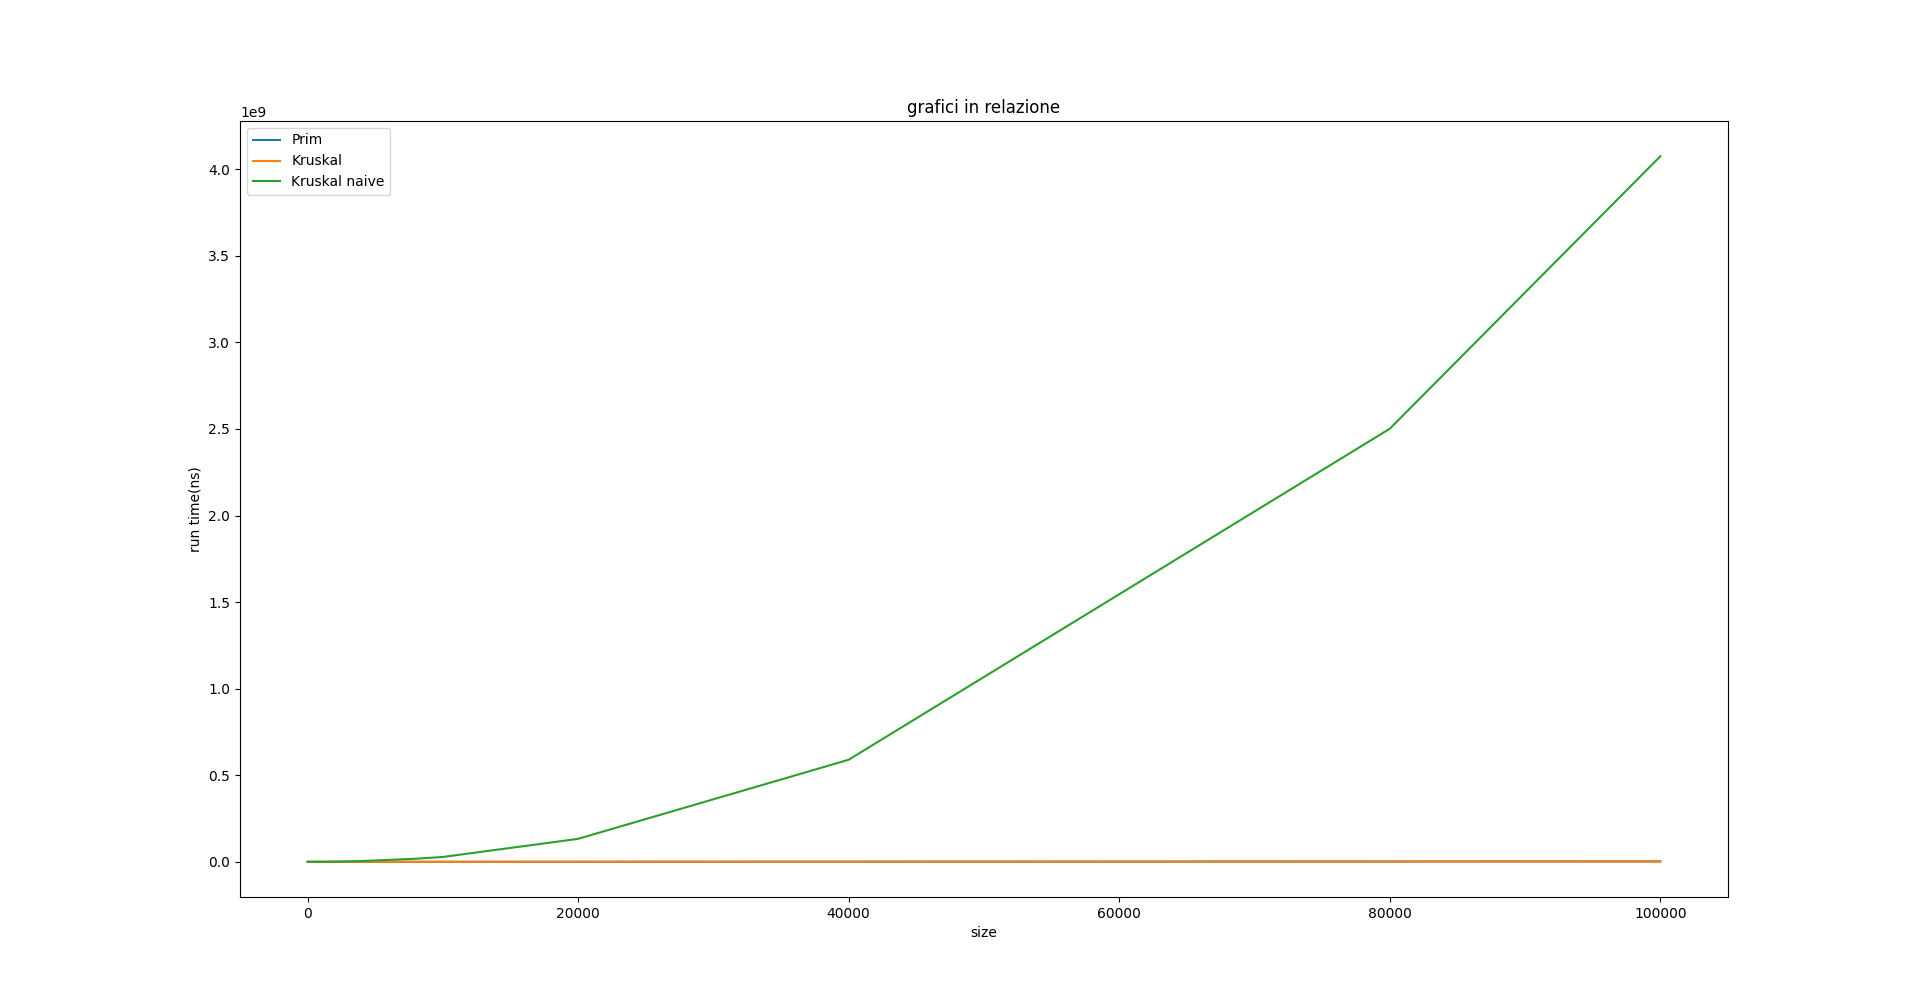
\includegraphics[scale = 0.38]{Fig/graficiRelazione.png}}
    \caption{grafico che mostra il confronto tra i 3 algoritmi: Naive Kruskal(verde), Kruskal(arancione), Prim(blu). Come si può notare dal grafico in figura 4, Kruskal naive cresce molto più velocemnte rispetto a Prim e Kruskal}
    \label{Kruskal naive}
\end{figure}

\newpage
\begin{figure}[htbp]
    \centering
    \centerline{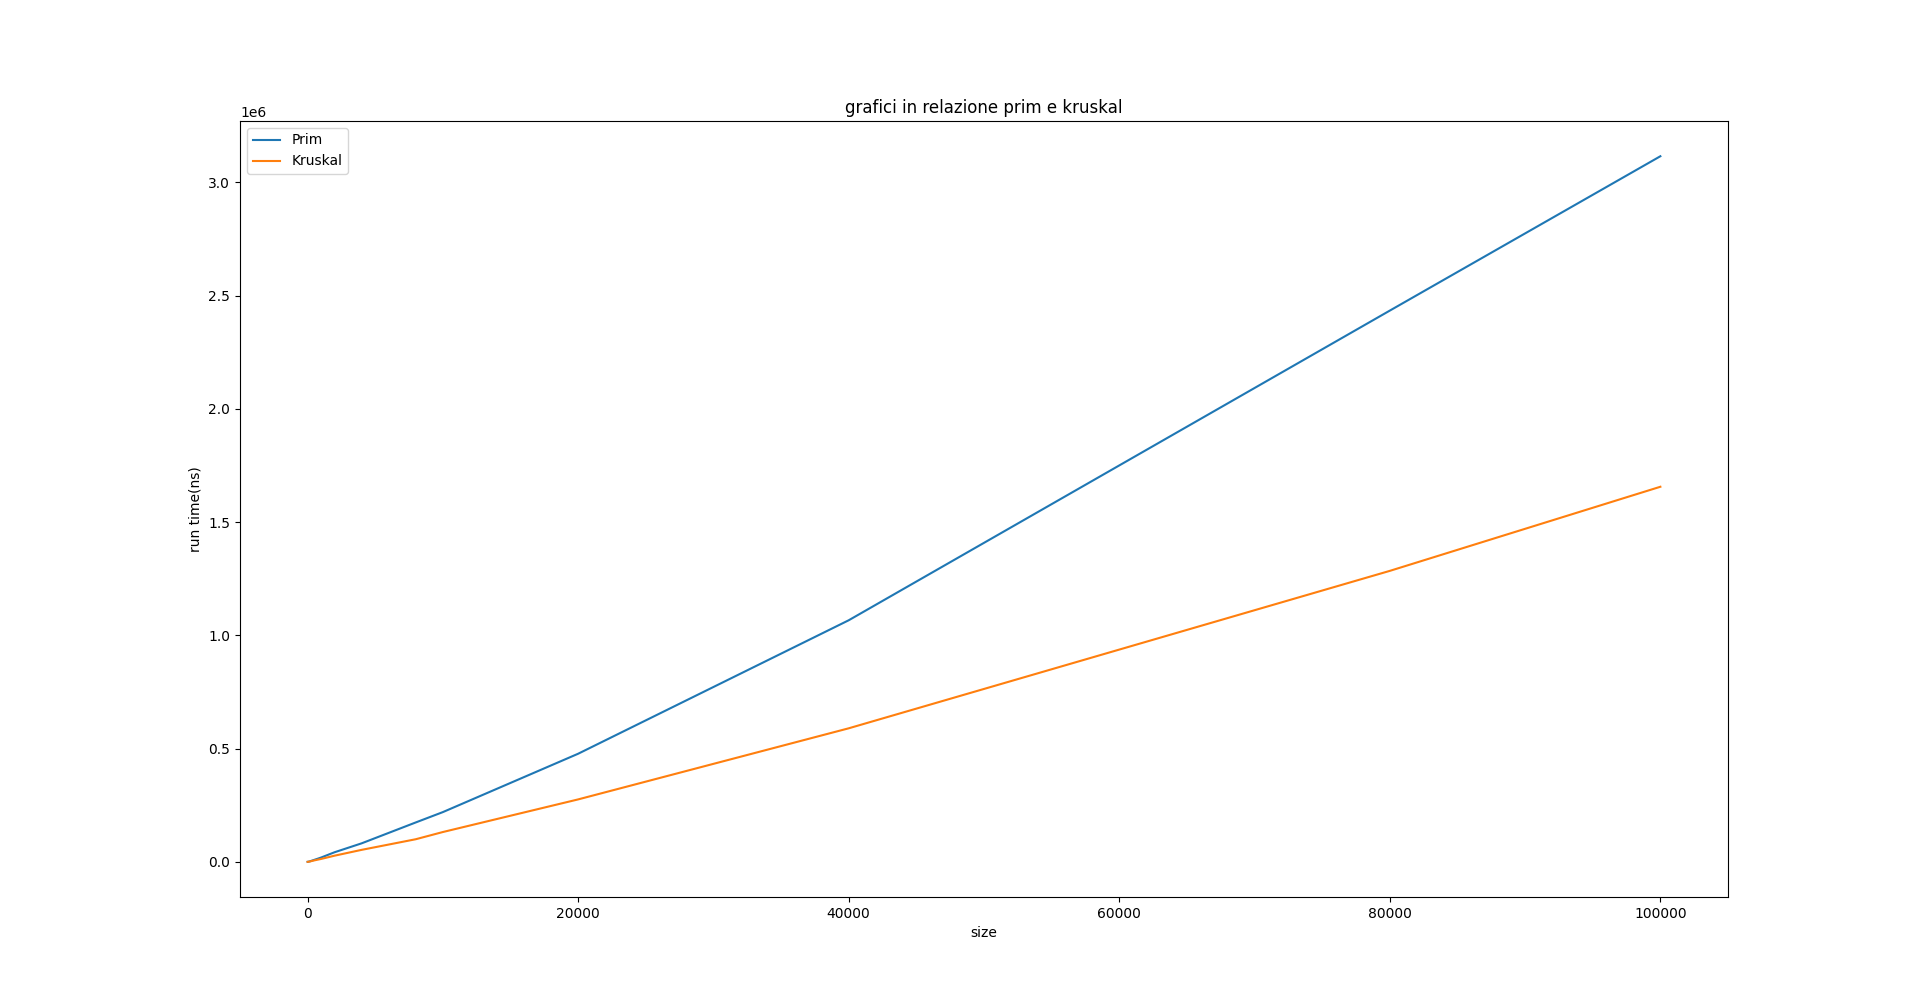
\includegraphics[scale = 0.38]{Fig/primkruskalrelazione.png}}
    \caption{grafico che mostra il confronto tra Prim(blu) e Kruskal(arancione)}
    \label{Kruskal naive}
\end{figure}

\newpage

\subsection{Tabella pesi}
\label{tabella\_pesi}

Di seguito viene riportata la tabella del calcolo dei pesi per ogni istanza divisi in base agli algoritmi. È possibile notare l'uguaglianza tra i pesi risultanti.

\rowcolors{2}{white!80!lightgray!90}{white}
\renewcommand{\arraystretch}{2}
\begin{longtable}[H]{|p{1.5cm}|p{1.5cm}|p{2cm}|p{3cm}|p{4cm}|} \hline
    \rowcolor{lightgray}
    \textbf{n\_nodi} & \textbf{n\_archi} & \textbf{peso Prim} & \textbf{peso Kruskal} & \textbf{peso Kruskal naive} \\ \hline\hline
    \endhead
    10 & 9 & 29316 & 29316 & 29316 \\ \hline
    10 & 10 & 25217 & 25217 & 25217 \\ \hline
    10 & 11 & 16940 & 16940 & 16940 \\ \hline
    10 & 13 & -44448 & -44448 & -44448 \\ \hline
    20 & 24 & -32021 & -32021 & -32021 \\ \hline 
    20 & 24 & 25130 & 25130 & 25130 \\ \hline
    20 & 26 & -37205 & -37205 & -37205 \\ \hline
    20 & 28 & -41693 & -41693 & -41693 \\ \hline
    40 & 50 & -31929 & -31929 & -31929 \\ \hline
    40 & 50 & -79570 & -79570 & -79570 \\ \hline
    40 & 52 & -79741 & -79741 & -79741 \\ \hline
    40 & 56 & -114203 & -114203 & -114203 \\ \hline
    80 & 99 & -198094 & -198094 & -198094 \\ \hline
    80 & 104 & -110571 & -110571 & -110571 \\ \hline
    80 & 108 & -139926 & -139926 & -139926 \\ \hline
    80 & 114 & -233320 & -233320 & -233320 \\ \hline
    100 & 129 & -271743 & -271743 & -271743 \\ \hline
    100 & 132 & -229506 & -229506 & -229506 \\ \hline
    100 & 136 & -141960 & -141960 & -141960 \\ \hline
    100 & 137 & -288906 & -288906 & -288906 \\ \hline
    200 & 267 & -393278 & -393278 & -393278 \\ \hline
    200 & 267 & -510185 & -510185 & -510185 \\ \hline
    200 & 269 & -444357 & -444357 & -444357 \\ \hline
    200 & 269 & -515136 & -515136 & -515136 \\ \hline
    400 & 518 & -788168 & -788168 & -788168 \\ \hline
    400 & 526 & -733645 & -733645 & -733645 \\ \hline
    400 & 538 & -895704 & -895704 & -895704 \\ \hline
    400 & 540 & -1119906 & -1119906 & -1119906 \\ \hline
    800 & 1049 & -1652119 & -1652119 & -1652119 \\ \hline 
    800 & 1058 & -1578294 & -1578294 & -1578294 \\ \hline 
    800 & 1063 & -1541291 & -1541291 & -1541291 \\ \hline
    800 & 1076 & -1664316 & -1664316 & -1664316 \\ \hline
    1000 & 1300 & -2089013 & -2089013 & -2089013 \\ \hline
    1000 & 1313 & -1934208 & -1934208 & -1934208 \\ \hline
    1000 & 1328 & -2229428 & -2229428 & -2229428 \\ \hline
    1000 & 1344 & -2356163 & -2356163 & -2356163 \\ \hline
    2000 & 2652 & -4717250 & -4717250 & -4717250 \\ \hline
    2000 & 2654 & -4739387 & -4739387 & -4739387 \\ \hline 
    2000 & 2677 & -4537267 & -4537267 & -4537267 \\ \hline 
    2000 & 2699 & -4811598 & -4811598 & -4811598 \\ \hline 
    4000 & 5315 & -9314968 & -9314968 & -9314968 \\ \hline
    4000 & 5340 & -9845767 & -9845767 & -9845767 \\ \hline
    4000 & 5360 & -8722212 & -8722212 & -8722212 \\ \hline
    4000 & 5368 & -8681447 & -8681447 & -8681447 \\ \hline 
    8000 & 10662 & -18741474 & -18741474 & -18741474 \\ \hline  
    8000 & 10670 & -18798446 & -18798446 & -18798446 \\ \hline  
    8000 & 10705 & -17844628 & -17844628 & -17844628 \\ \hline
    8000 & 10757 & -18178610 & -18178610 & -18178610 \\ \hline  
    10000 & 13287 & -22581384 & -22581384 & -22581384 \\ \hline
    10000 & 13301 & -22079522 & -22079522 & -22079522 \\ \hline
    10000 & 13311 & -22606313 & -22606313 & -22606313 \\ \hline
    10000 & 13340 & -22338561 & -22338561 & -22338561 \\ \hline 
    20000 & 26667 & -45962292 & -45962292 & -45962292 \\ \hline
    20000 & 26670 & -46418161 & -46418161 & -46418161 \\ \hline
    20000 & 26673 & -47854708 & -47854708 & -47854708 \\ \hline
    20000 & 26826 & -45195405 & -45195405 & -45195405 \\ \hline
    40000 & 53242 & -88771991 & -88771991 & -88771991 \\ \hline
    40000 & 53319 & -93017025 & -93017025 & -93017025 \\ \hline
    40000 & 53415 & -92003321 & -92003321 & -92003321 \\ \hline
    40000 & 53446 & -94397064 & -94397064 & -94397064 \\ \hline
    80000 & 106554 & -180793224 & -180793224 & -180793224 \\ \hline 
    80000 & 106586 & -182065015 & -182065015 & -182065015 \\ \hline 
    80000 & 106633 & -185997521 & -185997521 & -185997521 \\ \hline
    80000 & 106914 & -186834082 & -186834082 & -186834082 \\ \hline
    100000 & 133214 & -230168572 & -230168572 & -230168572 \\ \hline
    100000 & 133395 & -230698391 & -230698391 & -230698391 \\ \hline
    100000 & 133463 & -231011693 & -231011693 & -231011693 \\ \hline
    100000 & 133524 & -231393935 & -231393935 & -231393935  \\ \hline
\end{longtable}
\newpage
Di seguito invece è riportata la tabella con i tempi di esecuzione per ogni algoritmo e per ogni istanza. Si può notare come nelle prime istanze Prim performa meglio rispetto a Kruskal, anche se nelle istanze successiva ha sempre un tempo di esecuzione maggiore.
\subsection{Tabella tempi}
\label{tabella\_tempi}

\rowcolors{2}{white!80!lightgray!90}{white}
\renewcommand{\arraystretch}{2}
\begin{longtable}[H]{|p{1.5cm}|p{1.5cm}|p{2cm}|p{2cm}|p{3cm}|p{3cm}|} \hline
    \rowcolor{lightgray}
    \textbf{n\_nodi} & \textbf{n\_archi} & \textbf{Prim} & \textbf{Kruskal} & \textbf{Kruskal naive} & \textbf{alg. migliore}\\ \hline\hline
    \endhead
    10 & 9 & 37.0 & 43.0 & 66.0 & Prim : 37.0 \\ \hline
    10 & 10 & 34.0 & 45.0 & 78.0 & Prim : 34.0 \\ \hline
    10 & 11 & 42.0 & 46.0 & 64.0 & Prim : 42.0 \\ \hline
    10 & 13 & 37.0 & 50.0 & 79.0 & Prim : 37.0 \\ \hline
    20 & 24 & 98.0 & 101.0 & 207.0 & Prim : 98.0 \\ \hline
    20 & 24 & 92.0 & 109.0 & 236.0 & Prim : 92.0 \\ \hline
    20 & 26 & 104.0 & 111.0 & 213.0 & Prim : 104.0 \\ \hline
    20 & 28 & 105.0 & 132.0 & 294.0 & Prim : 105.0 \\ \hline
    40 & 50 & 244.0 & 230.0 & 606.0 & Kruskal : 230.0 \\ \hline
    40 & 50 & 282.0 & 236.0 & 592.0 & Kruskal : 236.0 \\ \hline
    40 & 52 & 249.0 & 244.0 & 545.0 & Kruskal : 244.0 \\ \hline
    40 & 56 & 264.0 & 243.0 & 587.0 & Kruskal : 243.0 \\ \hline
    80 & 99 & 603.0 & 499.0 & 2441.0 & Kruskal : 499.0 \\ \hline
    80 & 104 & 575.0 & 526.0 & 2178.0 & Kruskal : 526.0 \\ \hline
    80 & 108 & 639.0 & 521.0 & 2367.0 & Kruskal : 521.0 \\ \hline
    80 & 114 & 659.0 & 540.0 & 2956.0 & Kruskal : 540.0 \\ \hline
    100 & 129 & 810.0 & 642.0 & 2756.0 & Kruskal : 642.0 \\ \hline
    100 & 132 & 847.0 & 641.0 & 3031.0 & Kruskal : 641.0 \\ \hline
    100 & 136 & 814.0 & 673.0 & 3831.0 & Kruskal : 673.0 \\ \hline
    100 & 137 & 869.0 & 644.0 & 2518.0 & Kruskal : 644.0 \\ \hline
    200 & 267 & 2051.0 & 1604.0 & 13963.0 & Kruskal : 1604.0 \\ \hline 
    200 & 267 & 2011.0 & 1594.0 & 12516.0 & Kruskal : 1594.0 \\ \hline 
    200 & 269 & 2075.0 & 1589.0 & 10441.0 & Kruskal : 1589.0 \\ \hline 
    200 & 269 & 1946.0 & 1586.0 & 10749.0 & Kruskal : 1586.0 \\ \hline 
    400 & 518 & 4642.0 & 3274.0 & 36730.0 & Kruskal : 3274.0 \\ \hline 
    400 & 526 & 4814.0 & 3423.0 & 44668.0 & Kruskal : 3423.0 \\ \hline 
    400 & 538 & 4760.0 & 3872.0 & 41741.0 & Kruskal : 3872.0 \\ \hline 
    400 & 540 & 4748.0 & 3377.0 & 47742.0 & Kruskal : 3377.0 \\ \hline 
    800 & 1049 & 10668.0 & 7820.0 & 169127.0 & Kruskal : 7820.0 \\ \hline
    800 & 1058 & 10675.0 & 6827.0 & 164728.0 & Kruskal : 6827.0 \\ \hline
    800 & 1063 & 10913.0 & 7739.0 & 168908.0 & Kruskal : 7739.0 \\ \hline
    800 & 1076 & 10730.0 & 6873.0 & 164036.0 & Kruskal : 6873.0 \\ \hline
    1000 & 1300 & 14330.0 & 9562.0 & 248674.0 & Kruskal : 9562.0 \\ \hline
    1000 & 1313 & 13637.0 & 8709.0 & 271322.0 & Kruskal : 8709.0 \\ \hline
    1000 & 1328 & 13929.0 & 9082.0 & 269150.0 & Kruskal : 9082.0 \\ \hline
    1000 & 1344 & 14125.0 & 8976.0 & 259530.0 & Kruskal : 8976.0 \\ \hline
    2000 & 2652 & 30916.0 & 18345.0 & 1059458.0 & Kruskal : 18345.0 \\ \hline 
    2000 & 2654 & 31651.0 & 18992.0 & 1075133.0 & Kruskal : 18992.0 \\ \hline 
    2000 & 2677 & 32052.0 & 20291.0 & 1113125.0 & Kruskal : 20291.0 \\ \hline 
    2000 & 2699 & 31787.0 & 21161.0 & 1150464.0 & Kruskal : 21161.0 \\ \hline 
    4000 & 5315 & 71565.0 & 43781.0 & 4362490.0 & Kruskal : 43781.0 \\ \hline 
    4000 & 5340 & 70825.0 & 45548.0 & 4164992.0 & Kruskal : 45548.0 \\ \hline 
    4000 & 5360 & 70934.0 & 44696.0 & 4351926.0 & Kruskal : 44696.0 \\ \hline 
    4000 & 5368 & 72175.0 & 44362.0 & 4607022.0 & Kruskal : 44362.0 \\ \hline 
    8000 & 10662 & 153353.0 & 87139.0 & 17275593.0 & Kruskal : 87139.0 \\ \hline
    8000 & 10670 & 150470.0 & 87487.0 & 17472939.0 & Kruskal : 87487.0 \\ \hline
    8000 & 10705 & 155038.0 & 90897.0 & 19034256.0 & Kruskal : 90897.0 \\ \hline
    8000 & 10757 & 152228.0 & 88914.0 & 17995782.0 & Kruskal : 88914.0 \\ \hline
    10000 & 13287 & 199069.0 & 114678.0 & 27519384.0 & Kruskal : 114678.0 \\ \hline 
    10000 & 13301 & 198213.0 & 114541.0 & 28212040.0 & Kruskal : 114541.0 \\ \hline 
    10000 & 13311 & 198148.0 & 114831.0 & 28410336.0 & Kruskal : 114831.0 \\ \hline 
    10000 & 13340 & 200183.0 & 115300.0 & 28169334.0 & Kruskal : 115300.0 \\ \hline 
    20000 & 26667 & 460829.0 & 247868.0 & 135050130.0 & Kruskal : 247868.0 \\ \hline
    20000 & 26670 & 466592.0 & 240454.0 & 131505987.0 & Kruskal : 240454.0 \\ \hline
    20000 & 26673 & 461937.0 & 245921.0 & 131375244.0 & Kruskal : 245921.0 \\ \hline
    20000 & 26826 & 505290.0 & 243914.0 & 133029623.0 & Kruskal : 243914.0 \\ \hline
    40000 & 53242 & 1052767.0 & 539613.0 & 582092711.0 & Kruskal : 539613.0 \\ \hline 
    40000 & 53319 & 1017180.0 & 530200.0 & 579462411.0 & Kruskal : 530200.0 \\ \hline 
    40000 & 53415 & 962333.0 & 541707.0 & 602520927.0 & Kruskal : 541707.0 \\ \hline 
    40000 & 53446 & 967208.0 & 537543.0 & 594354801.0 & Kruskal : 537543.0 \\ \hline 
    80000 & 106554 & 2246350.0 & 1180804.0 & 2484800866.0 & Kruskal : 1180804.0 \\ \hline
    80000 & 106586 & 2131476.0 & 1175085.0 & 2497156786.0 & Kruskal : 1175085.0 \\ \hline
    80000 & 106633 & 2148715.0 & 1172859.0 & 2503001407.0 & Kruskal : 1172859.0 \\ \hline
    80000 & 106914 & 2213052.0 & 1178719.0 & 2520653034.0 & Kruskal : 1178719.0 \\ \hline
    100000 & 133214 & 2769982.0 & 1537615.0 & 4041731255.0 & Kruskal : 1537615.0 \\ \hline 
    100000 & 133395 & 2761894.0 & 1533403.0 & 4099202631.0 & Kruskal : 1533403.0 \\ \hline 
    100000 & 133463 & 2738139.0 & 1531136.0 & 4041570425.0 & Kruskal : 1531136.0 \\ \hline 
    100000 & 133524 & 2743588.0 & 1528937.0 & 4118205760.0 & Kruskal : 1528937.0 \\ \hline 
\end{longtable}









